Le bruit de Perlin est très utilisé dans la génération d'image. Effet, ce bruit permet de déterminer une élévation d'un sommet de N-dimension (dans notre cas 3). Nous avons donc implémenté un algorithme de afin de générer. L'algorithme se divise en deux temps :

\begin{enumerate}
	\item Initialisation
	\item Calcul
\end{enumerate}

La phase d'initialisation consite à avoir un tableau de 512 éléments bien mélangés compris entre 0 et 255. Enfin, le tableau se répète à partir de la valeur 256 (tab[0] = tab[256], et ainsi de suite). La phase de calcul est plus compliquée, car elle se découpe en plusieurs étapes. Le principe de l'algorithme est de retourner une même valeur en fonction d'un x, d'un y, et d'un z donné. On place x, y , z dans l'interval [0;255] avec un "et" logique. Ensuite on calcul les coordonnées en gradient du cube dans l'espace. Enfin, on calcul la valeur de retour. Ken Perlin a ensuite amélioré cet algorithme, afin qu'il soit plus performant en terme de calcul et de résultat. Cette version s'appelle le bruit de simplex.

Afin de générer aléatoirement un monde virtuel, il est necessaire de remplir le tableau aléatoirement à chaque démarrage du projet. En effet, sinon on obtiendra toujours la même monde carte, car le tableau de permutation reste toujours le même entre deux chargements.

Voici le monde que l'on a reussi à généré :

\begin{center}
	\null\vspace{0.25cm}
	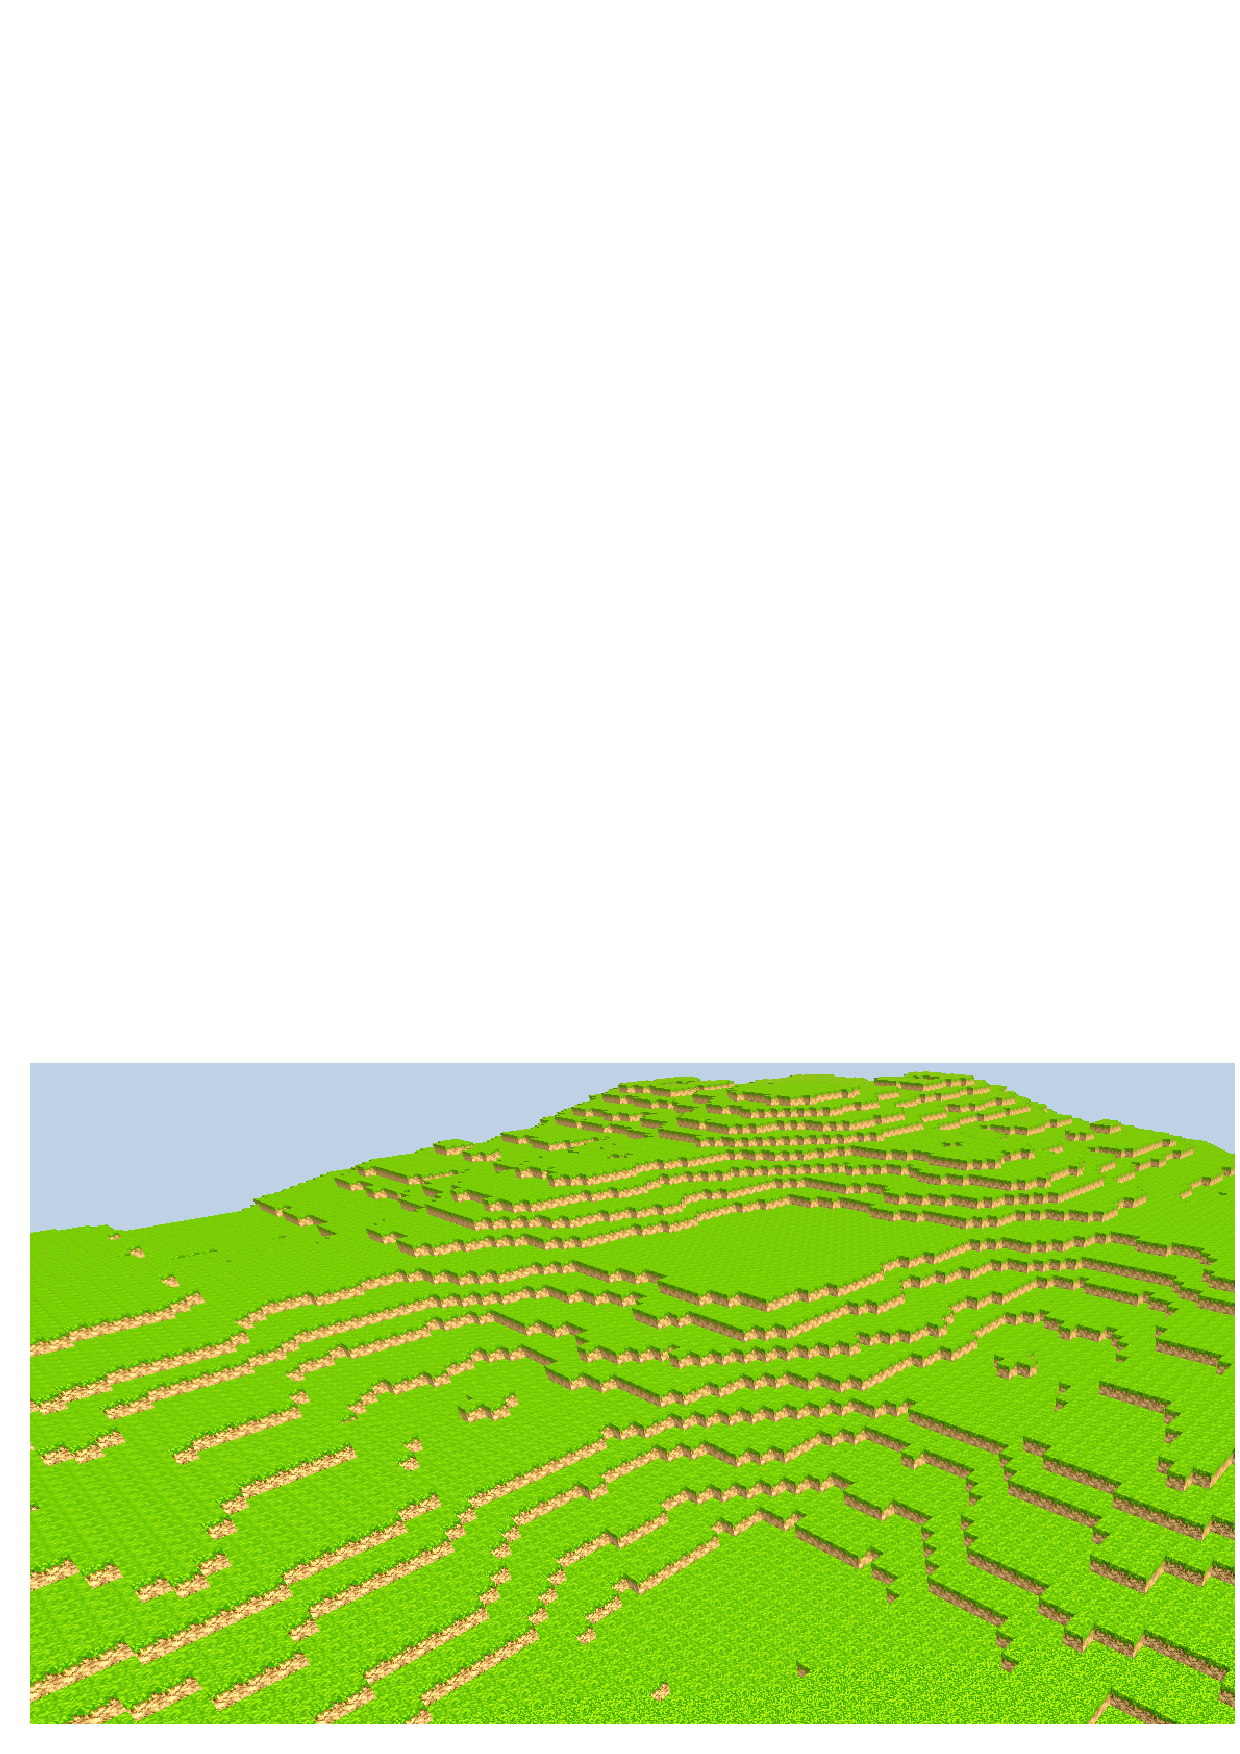
\includegraphics[height=3cm]{images/OurMinecraftWorld.png}\\
	\textit{Monde que l'on a généré à partir de l'exemple de l'API three.JS}\\
\end{center}